\documentclass{article}
\usepackage[utf8x]{inputenc}
\usepackage{graphicx}
\usepackage{amsmath}
\usepackage{amssymb}
\usepackage{tikz}
\usepackage{todonotes}
\usepackage{pgfplots}
\usepackage{epstopdf}
\usepackage{listings}
\usepackage{circuitikz}
\usepackage{float}
\usepackage{cleveref}
\usepackage{ragged2e} % For text alignment


\newenvironment{custom_itemize}{
\begin{itemize}
  \setlength{\itemsep}{0pt}
  \setlength{\parskip}{0pt}
  \setlength{\parsep}{0pt}
}{\end{itemize}}


\usepackage[hmarginratio=1:1,top=22mm,columnsep=16pt]{geometry} % Document margins
%\usepackage{multicol} % Used for the two-column layout of the document


%\usepackage{bm}


\title{NASA project}
\author{Kees Kroep 4246373}


\begin{document}
%  \twocolumn[{%
% \begin{@twocolumnfalse}
%  \maketitle
%   \end{@twocolumnfalse}
% }]


\newpage

\begin{figure}[h]
	\centering
	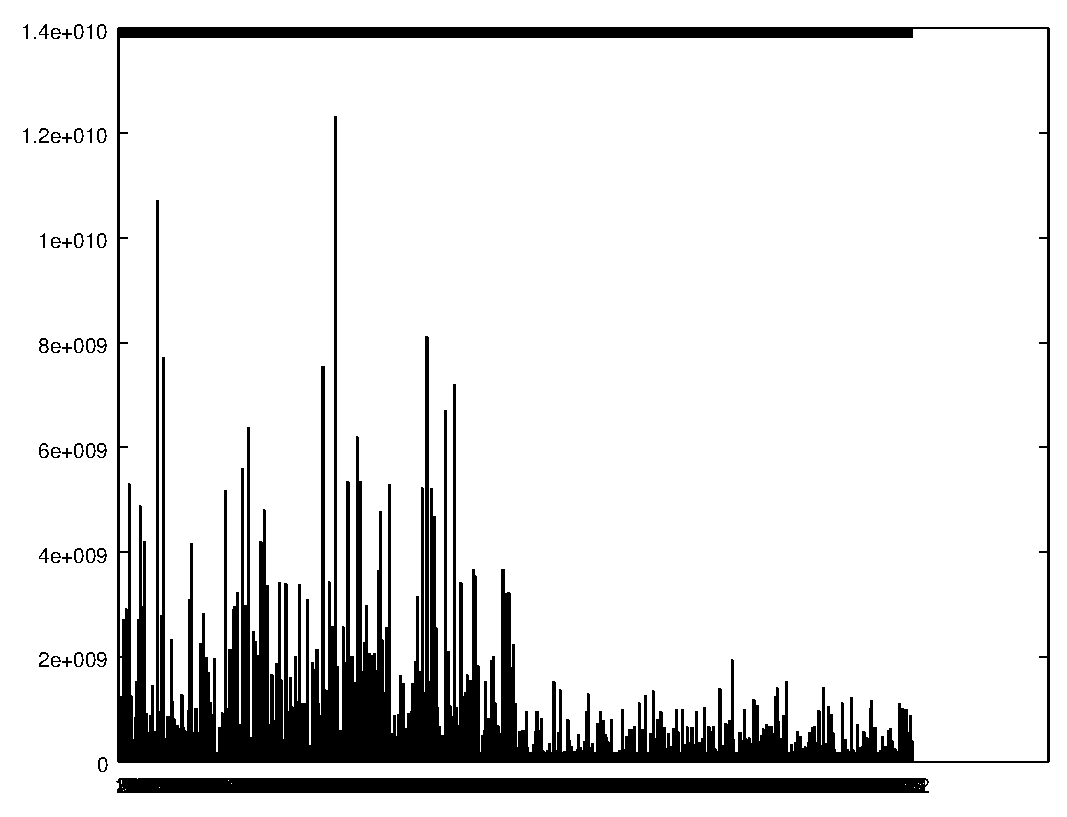
\includegraphics{measurement/bars}
	\caption{bars
	}
	\label{fig:bars}
\end{figure}


\begin{figure}[h]
	\centering
	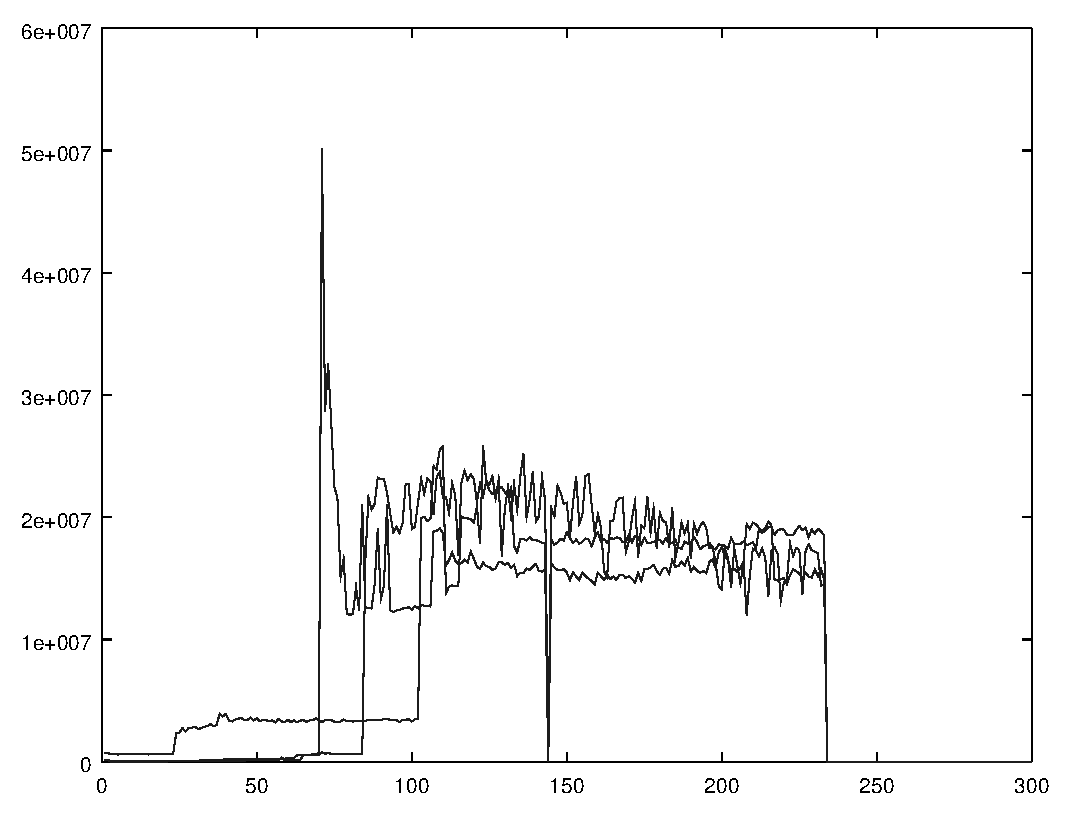
\includegraphics{measurement/spad_high}
	\caption{spad high}
	\label{fig:spad_high}
\end{figure}


\begin{figure}[h]
	\centering
	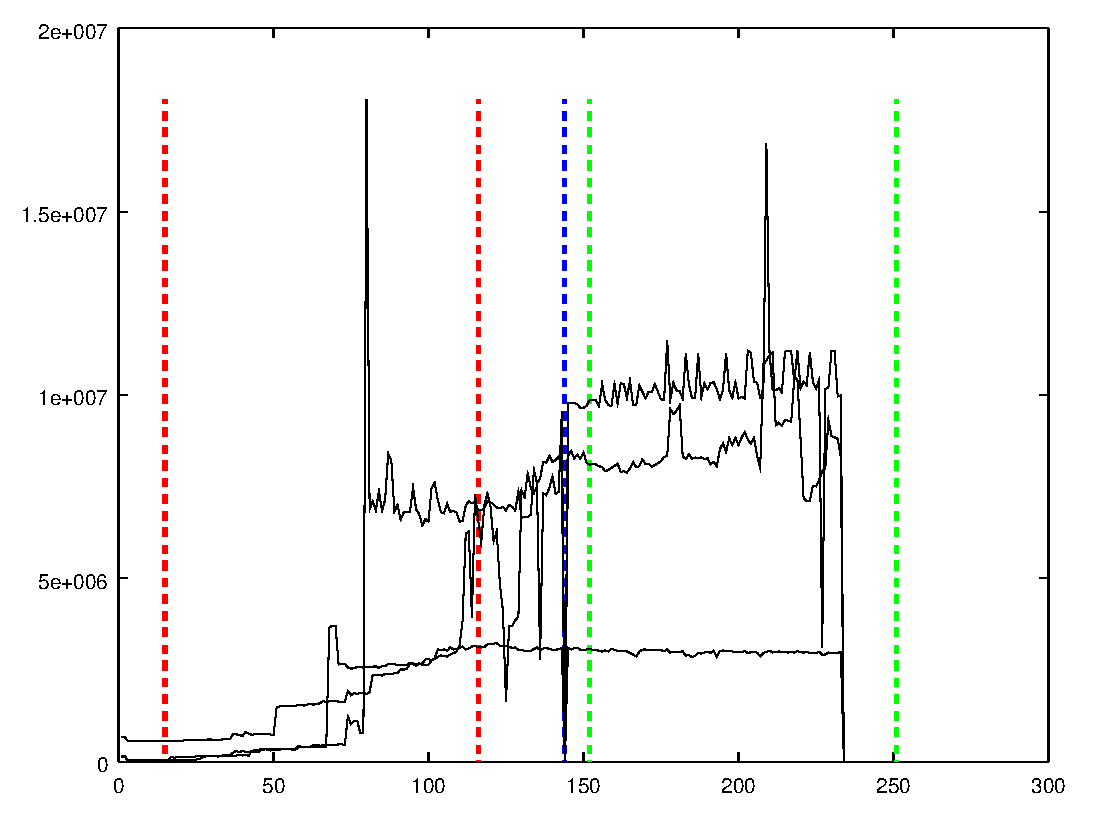
\includegraphics{measurement/spad_mid}
	\caption{spad mid}
	\label{fig:spad_mid}
\end{figure}

\begin{figure}[h]
	\centering
	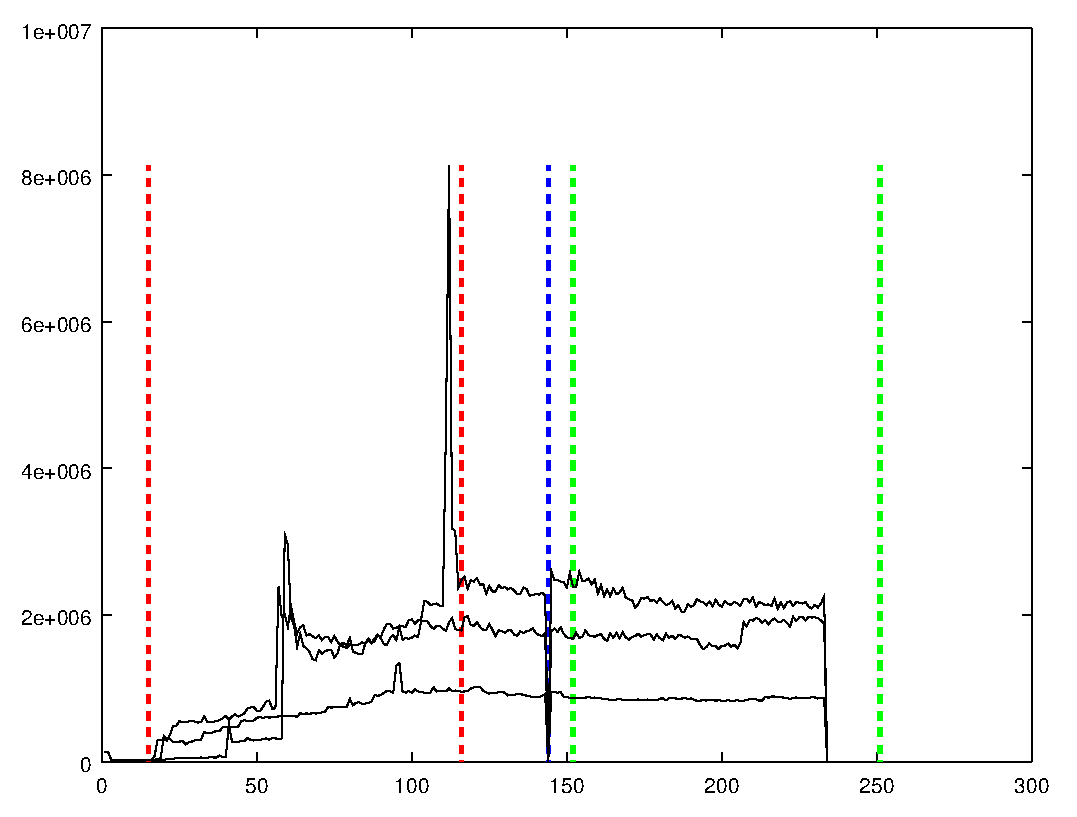
\includegraphics{measurement/spad_low}
	\caption{spad low}
	\label{fig:spad_low}
\end{figure}








\end{document}












